\documentclass[preview]{standalone}

\usepackage{amsmath}
\usepackage{amssymb}
\usepackage{stellar}
\usepackage{definitions}
\usepackage{tikz}

\begin{document}

\id{conic-sections}
\genpage

\section{Conic sections}

\begin{snippetdefinition}{conic-section-definition}{Conic section}
    A \textit{conic section} is the curve formed by the intersection of a right circular cone with a plane.
\end{snippetdefinition}

\begin{snippet}{conic-sections-illustration}
    \begin{center}
    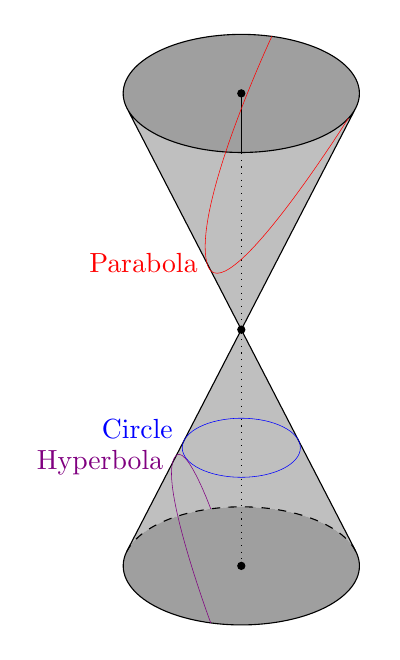
\begin{tikzpicture}[scale=1.5,parabola/.style={very thin, red}, hyperbola/.style={very thin, violet}, circle/.style={very thin, blue}]
        \def\b{2}
        \def\h{2}
        \def\p{0.5}
        \pgfmathsetmacro{\rx}{\b/2}
        \pgfmathsetmacro{\ry}{\rx*\p}
        \pgfmathsetmacro{\ta}{90-atan2(\h,\ry)}
        \fill[gray!50]
        (0, \h) -- (\ta:\rx+0 and \ry) arc (\ta:180-\ta:\rx+0 and \ry) -- cycle;
        \fill[gray!75] coordinate (bottom) ellipse [x radius=\rx, y radius=\ry];
        \draw[dashed] (\ta:\rx+0 and \ry) arc (\ta:180-\ta:\rx+0 and \ry);
        \draw (0, \h) -- (\ta:\rx+0 and \ry) arc (\ta:-180-\ta:\rx+0 and \ry) -- coordinate[pos=.4](hypbend) cycle;
        \begin{scope}[rotate around={180:(0,\h)}]
        \fill[gray!50]
        (0, \h) -- (\ta:\rx+0 and \ry) arc (\ta:180-\ta:\rx+0 and \ry) -- cycle;
        \fill[gray!75] coordinate (top) ellipse [x radius=\rx, y radius=\ry];
        \draw (\ta:\rx+0 and \ry) arc (\ta:180-\ta:\rx+0 and \ry) (0, \h) -- coordinate[pos=.3](parabend) (\ta:\rx+0 and \ry) arc (\ta:-180-\ta:\rx+0 and \ry) -- cycle;
        \end{scope}
        %% Dots & Axis
        \fill (top) circle[radius=1pt] (0,\h) circle[radius=1pt] (bottom) circle[radius=1pt];
        \draw[dotted] (top) -- (bottom);
        \draw (top) -- ++(-90:\rx+0 and \ry);
        %% Parabola
        \path (top) +(50+50*\p:\rx+0 and \ry) coordinate (tmp) +(-50+50*\p:\rx+0 and \ry) coordinate (tmp2);
        \draw[parabola] (tmp) ..controls ++(-90:0) and ++(\ta+90:\p).. (parabend) node[left]{Parabola} ..controls ++(\ta-90:\p) and ++(-90:0).. (tmp2);
        %% Circle
        \def\pos{0.5}
        \draw[circle] (0,\pos*\h) ellipse [x radius=\pos*\rx, y radius=\pos*\ry] +(180:\pos*\rx) node[above left]{Circle};
        %% Hyperbola
        \path (bottom) +(130-50*\p:\rx+0 and \ry) coordinate (tmp) +(230+50*\p:\rx+0 and \ry) coordinate (tmp2);
        \draw[hyperbola] (tmp) ..controls ++(90:0) and ++(90-\ta:0.6*\p).. (hypbend) node[left]{Hyperbola} ..controls ++(-\ta-90:0.6*\p) and ++(90:0).. (tmp2);
    \end{tikzpicture}
    \end{center}
\end{snippet}

\plain{The conic sections are circles, ellipses, parabolas and hyperbolas.}

\end{document}